\section{Dual-Learning Fault Localization}

\begin{figure}[t]
	\centering
	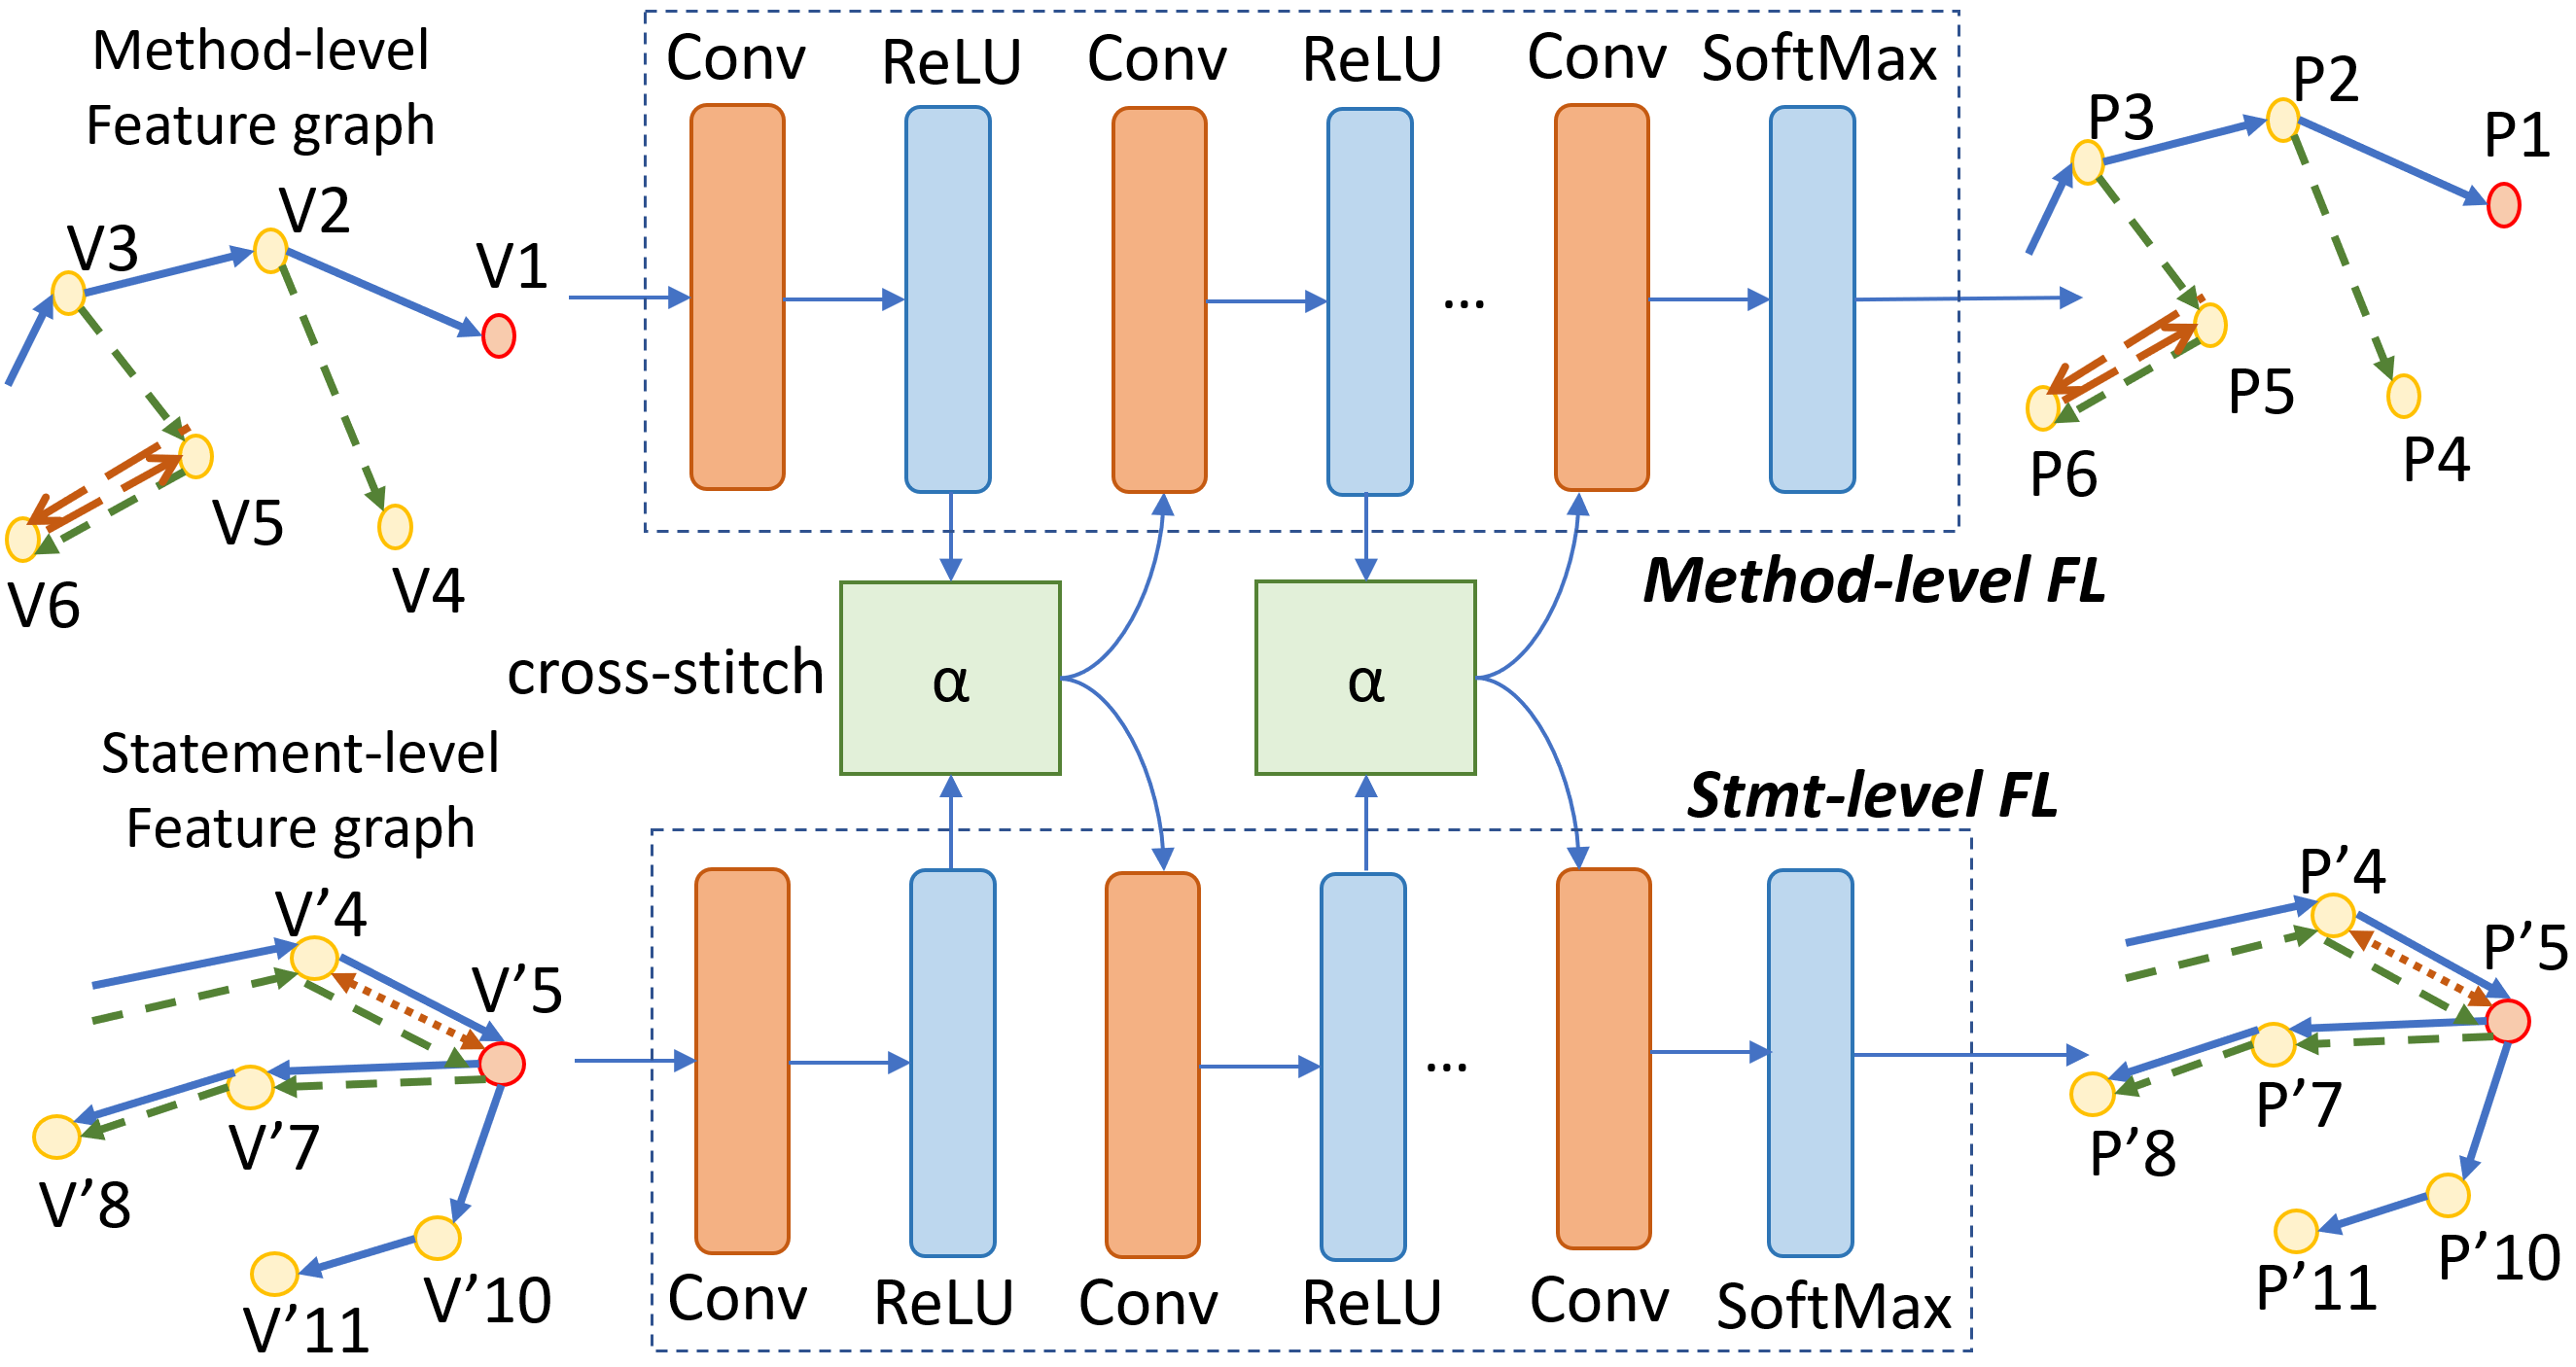
\includegraphics[width=3in]{graphs/dual-learning.png}
	\caption{Dual-Learning Fault Localization}
	\label{dual-learning}
\end{figure}


After having the vectorized graph $G_m$ and $G_s$ for both the method-level and the statement-level features, in this step, \tool applies a dual learning fault localization model to extract the fault locations. So there are two main tasks in this step, including the method-level fault localization and the statement-level fault localization. So the input for this step is the two graphs $G_m$ and $G_s$, and the expected output is the prediction label for each node in these two graphs from these two tasks.

Specifically, \tool firstly builds two separate GCN models \cite{kipf2016semi} for the method-level fault localization and the statement-level fault localization. For the GCN model applied on the method-level, there are $i$ graph convolutional layer $Conv_1, Conv_2, ..., Conv_i$ as shown in Figure \ref{dual-learning} and after each graph convolutional layer $Conv_i$, there is $ReLU$ layer follows it. Considering a graph convolutional layer $Conv_i$ and the following $ReLU$ layer together as one big layer, the GCN model contains $i$ layers in total. The only special case is in the last layer. There is a $SoftMax$ layer following the graph convolutional layer instead of a $RuLU$ layer. Similar to the GCN model applied on the method-level, for the statement-level fault location, there is the other GCN model with $i$ layers. Each layer contains one graph convolutional layer $Conv'_i$ and one $Relu$ layer. And the $SoftMax$ layer replaces the $ReLU$ layer in the last layer of the GCN model.

To achieve the information sharing between two layers as a dual learning framework, we use the cross-stitch unit \cite{misra2016cross} for help. To be more detailed, for each layer of GCN, it calculates the hidden status using the following formula.

\begin{equation}\label{eq:1}
	\hat{A} = D'^{-\frac{1}{2}}A'D'{-\frac{1}{2}}
\end{equation}

\begin{equation}\label{eq:2}
	H_i = \Delta(\hat{A}X_iW_i)
\end{equation}

Where $A'$ is the adjacency matrix; $D'$ is the degree matrix; $W_i$ is the weight matrix for layer $i$; $X_i$ is the input for layer $i$; $H_i$ is the hidden status of layer $i$; and $\Delta$ is the activation function $ReLU$. $H_i$ here is the output from the $ReLU$ layer and will be regarded as the input of the next layer of GCN. The cross-stitch unit is suitable to be added here.

As seen in Figure \ref{dual-learning}, after the $ReLU$ layers we have $H_i^m$ and $H_i^s$ as the method-level and the statement-level hidden status. By putting them all into the cross-stitch unit, we have:

\begin{equation}\label{eq:3}
	\begin{bmatrix}
		W_{m,m} &  W_{m,s} \\
		W_{s,m} &  W_{s,s}
	\end{bmatrix}
	\begin{bmatrix}
		H_m^{i}\\
		H_s^{i}
	\end{bmatrix}=
	\begin{bmatrix}
		X_m^{i+1}\\
		X_s^{i+1}
	\end{bmatrix}
\end{equation}

Where $W$ is the trainable or preset weight matrix, in \tool, we make it as the trainable weights; $X$ is the input for the $i+1$ layer of GCN. So with the cross-stitch unit, \tool gets $X_m^{i+1}$ and $X_s^{i+1}$ in this step as the input for the $i+1$ layer instead of directly feed $H_i^m$ and $H_i^s$ into the $i+1$ layer as input. The $X_m^{i+1}$ and $X_s^{i+1}$ contains the information learned from both the method-level and the statement-level that can help achieve the main goal for dual learning to enhance the performance of fault localization on both levels.

But one special situation \tool may face in the cross-stitch unit is that the size of the outputs $H_i^m$ and $H_i^s$ from layer $i$ may be different. The different size of matrix will make the cross-stitch unit not work as expected. To avoid this problem, \tool resizes the matrix to make the process work. To be more detailed, from formula \ref{eq:3} we can know that:

\begin{equation}\label{eq:4}
	X_m^{i+1} = W_{m,m}H_m^{i} + W_{m,s}H_s^{i}
\end{equation}
\begin{equation}\label{eq:5}
	X_s^{i+1} = W_{s,m}H_m^{i} + W_{s,s}H_s^{i}
\end{equation}

Within formula \ref{eq:4} and \ref{eq:5}, \tool would like to resize $H_s^{i}$ in formula \ref{eq:4} and resize $H_m^{i}$ in formula \ref{eq:5}. If the matrix size needed to be increased, \tool uses a well-known image processing technique, bilinear interpolation, to help solve this problem. Firstly, \tool pads zeros to the matrix to make the aspect ratio be $1:1$. And then \tool uses the bilinear interpolation to resize the matrix. If the matrix size needed to be reduced, \tool does the center crop on the matrix to match the required size.

By solving this problem, the cross-stitch unit can help share the information between two GCN models for both the method-level and the statement-level fault localization. The dual-learning fault localization model accepts the vectorized graphs as input and generates the label for each node. And there is a trainable threshold to determine if the node belongs to the $buggy$ class or the $non-buggy$ class. Thus, by collecting all nodes marked as $buggy$, \tool regards this set of predicted $buggy$ methods/statements as the output. 

